\documentclass[a4paper]{report}
\usepackage[utf8]{inputenc}
\usepackage{amsmath}
\usepackage{esint}
\usepackage{tabstackengine}
\usepackage[colorlinks,linkcolor=blue]{hyperref}
\usepackage{xeCJK}
\usepackage{mathrsfs}
\usepackage{commath}
\usepackage{tikz}
\usepackage{float}
\usetikzlibrary{calc}
\usepackage{pgfplots}
\usepackage{mathrsfs}
\usepackage{amsfonts}
\usetikzlibrary{arrows}
\usepackage{pgf,tikz,pgfplots}
\usepackage{ulem}
\usepackage{enumitem}
\setlist[1]{itemsep=-5pt}

%%%% 下面的命令重定义页面边距,使其符合中文刊物习惯 %%%%
\addtolength{\topmargin}{-54pt}
\setlength{\oddsidemargin}{0.63cm}  % 3.17cm - 1 inch
\setlength{\evensidemargin}{\oddsidemargin}
\setlength{\textwidth}{14.66cm}
\setlength{\textheight}{24.00cm}    % 24.62

%%%% 段落首行缩进两个字 %%%%
% \makeatletter
% \let\@afterindentfalse\@afterindenttrue
% \@afterindenttrue
% \makeatother
% \setlength{\parindent}{2em}  %中文缩进两个汉字位

% 段首不缩进
\setlength{\parindent}{0pt}
%%%% 下面的命令设置行间距与段落间距 %%%%
\linespread{1.4}
% \setlength{\parskip}{1ex}
\setlength{\parskip}{0.5\baselineskip}


\title{Note}
\author{Crosstyan}
\date{July 2020}

\begin{document}

%\maketitle

\chapter{Vector Analyse}


\section{Basic Theorem}
\subsection{Divergence Theorem}
$$ \iiint_{V} (\nabla\cdot\vec{F})\,dV=\oiint_S\vec{F}\,d\vec{A}$$
\subsection{Stokes Theorem}
$$ \iint_{S}(\nabla\times\vec{F})\,d\vec{A}=\oint_l\vec{F}\,d\vec{l} $$
\section{Coords}
\subsection{Cylindrical Coordinate}
\subsubsection{Line Element}
$$d\vec{r}=d\rho\cdot\hat{\rho}+\rho\;d\phi \cdot\hat{\phi}+dz\cdot \hat{z}$$
\subsubsection{Surface Element}
\begin{align*}
    d\vec{S}&=\hat{\rho}\cdot dS_\rho+\hat{\phi}\cdot dS_\phi+\hat{z}\cdot dS_z\\
    dS_\rho&=\rho\;d\phi\;dz\\
    dS_\phi&=d\rho dz\\
    dS_z&=\rho\;d\rho\; d\phi
\end{align*}
\subsubsection{Volume Element}
$$dV=\rho\;d\rho\;dz$$
\subsubsection{Conversion}
from Cartesian
\begin{align*}
    \rho&=\sqrt{x^2+y^2}\\
    \phi&=\arctan(\frac{y}{x})\\
    z&=z
\end{align*}
to Cartesian
\begin{align*}
    x&=\rho\cdot \cos(\phi)\\
    y&=\rho \cdot \sin(\phi)\\
    z&=z
\end{align*}
\subsection{Spherical Coordinate}
\subsubsection{Line Element}
$$d\vec{r}=dr\cdot\hat{r}+r\cdot d\theta\cdot \hat{\theta}+r\cdot \sin(\theta)\cdot d\phi\cdot \hat{\phi}$$
\subsubsection{Surface Element}
$$d\vec{S}=\hat{r}\cdot dS_r+\hat{\phi}\cdot dS_\phi+\hat{\theta}\cdot dS_\theta$$
Radius r is constant. 
$$dS_r=r^2\cdot\sin(\theta)\cdot d\theta\;d\phi$$
Polar Angle ($\theta$) is constant. 
$$ dS_\theta=r\;\sin(\theta)\;d\phi\;d\theta $$
Azimuth ($\phi$) is constant. 
$$dS_\phi=r\cdot dr\;d\theta$$
\subsubsection{Volume Element}
$$dV=r^2\;\sin(\theta)\;dr\;d\theta\;d\phi$$
\subsubsection{Conversion}
from Cartesian
\begin{align*}
    r&=\sqrt{x^2+y^2+z^2}\\
    \theta&=arctan(\frac{\sqrt{x^2+y^2}}{z})\\
    \phi&=arctan(\frac{y}{x})
\end{align*}
to Cartesian
\begin{align*}
    x&=r\;\sin(\theta)\;\cos(\phi)\\
    y&=r\;\sin(\theta)\;\sin(\phi)\\
    z&=r\;\cos(\theta)
\end{align*}
from Cylindrical
\begin{align*}
    r&=\sqrt{\rho^2+z^2}\\
    \theta&=arctan(\frac{\rho}{z})\\
    \phi&=\phi
\end{align*}
\section{Grad, Divergence and Curl}
%Table of Coords
\begin{table}[h]
  \centering
  \begin{tabular}{c c c c}
    Coords&Cartesian&Cylindrical&Spherical \\
    $q_1$&x&$\rho$&r \\
    $q_2$&y&$\phi$&$\theta$ \\
    $q_3$&z&z&$\phi$ \\
    \hline
    $h_1$&1&1&1 \\
    $h_2$&1&$\rho$&r \\
    $h_3$&1&1&$r\cdot\sin(\theta)$ \\
  \end{tabular}
  \caption{Table of Coords}
\end{table}
\subsection{Line Element}
$$d\vec{l}=h_1dq_1\cdot\hat{q_1}+h_2dq_2\cdot\hat{q_2}+h_3dq_3\cdot\hat{q_3}$$
\subsection{Gradient}
\renewcommand{\arraystretch}{2}
$$
\nabla f=
\begin{bmatrix}
    \frac{1}{h_1}\cdot\frac{\partial f}{\partial q_1}\\
    \frac{1}{h_2}\cdot\frac{\partial f}{\partial q_2}\\
    \frac{1}{h_3}\cdot\frac{\partial f}{\partial q_3}
\end{bmatrix}\cdot
\begin{bmatrix}
    \hat{q_1}\\
    \hat{q_2}\\
    \hat{q_3}
\end{bmatrix}
$$
\subsection{Divergence}
Let's say that $\vec{F}=F_1\cdot\hat{q_1}+F_2\cdot\hat{q_2}+F_3\cdot\hat{q_3}$
$$
\nabla\cdot\vec{F}=
\frac{1}{h_1h_2h_3}\cdot
\left[
    \frac{\partial
    \left(
        F_1\cdot h_2 h_3
    \right)}{\partial q_1}
    +
    \frac{\partial
    \left(
        F_2\cdot h_1 h_3
    \right)}{\partial q_2}
    +
    \frac{\partial
    \left(
        F_3\cdot h_1 h_2
    \right)}{\partial q_3}
\right]
$$
\subsection{Curl}
Let's say that $\vec{F}=F_1\cdot\hat{q_1}+F_2\cdot\hat{q_2}+F_3\cdot\hat{q_3}$
$$
\nabla\times\vec{F}=
\frac{1}{h_1h_2h_3}
\cdot
\begin{vmatrix}
    h_1\hat{q_1}&h_2\hat{q_2}&h_2\hat{q_3}\\
    \frac{\partial}{\partial q_1}&\frac{\partial}{\partial q_2}&\frac{\partial}{\partial q_3}\\
    h_1\cdot F_1&h_2\cdot F_2&h_3\cdot F_3
\end{vmatrix}
$$
\subsection{Laplacian}
$$ 
    \nabla^2 f = \nabla\cdot\nabla f
$$
%$$\nabla^2 f=\frac{1}{h_1 h_2 h_3} $$
\section{恒等式}
\subsection{The curl of grad equals 0}
$$\nabla\times (\nabla f)=0$$
如果一个矢量场的旋度为0, 那么该场可以表示为一个标量场的梯度. 
\subsection{The divergence of curl equals 0}
$$\nabla\cdot (\nabla\times \vec{A})=0$$
一个矢量场的散度为0, 则该场可以表示为一个矢量场的旋度. 
\subsection{分配律}
标量与标量和
$$\nabla\cdot (f\vec{A})=f \underset{\text{div of $\vec{A}$ is scale}}{\nabla\cdot \vec{A}} + \underset{\text{矢量与矢量点乘为标量且$\nabla f$是矢量}}{\vec{A}\cdot \nabla f}$$
矢量与矢量和
$$\nabla\times (f\vec{G})=\underset{\text{标量乘上矢量仍然为矢量}}{f} \nabla\times \vec{G}+\underset{\text{矢量叉乘为矢量}}{\nabla f \times \vec{G}} $$
矢量与矢量和
$$\nabla(fg)=f\nabla g+g\nabla f$$
\section{Helmholtz decomposition}
$ \vec{F} $ can be decomposed to divergence-less (like $ \vec{B} $) and curl-less (like $ \vec{E} $). 
$$ \vec{F}= -\nabla\phi+\nabla\times\vec{A} $$
在此$\phi$即标量电位, $\vec{A}$为矢量磁位. 
\chapter{Maxwell's Equation}
\section{Differential equations}
$$
\begin{cases}
    \nabla\times \vec{H} =\vec{J}_{\text{free}}+\frac{\partial \vec{D} }{\partial t}\\
    \nabla\times \vec{E} =-\frac{\partial \vec{B} }{\partial t}\\
    \nabla\cdot \vec{B} =0\\
    \nabla\cdot \vec{D} =\rho_{\text{free}}\\
\end{cases}
$$
\subsection{Ampère's circuital law (with Maxwell's addition)}
$$\nabla\times \vec{H} =\vec{J}+\frac{\partial \vec{D} }{\partial t}$$
时变电场由传导电流和位移电流产生, 时变电场(RHS)产生时变磁场(LHS)
\subsection{Maxwell–Faraday equation (Faraday's law of induction)}
$$\nabla\times \vec{E} =-\frac{\partial \vec{B} }{\partial t}$$
时变磁场(RHS)产生时变电场(LHS)
\subsection{Gauss's law for magnetism}
$$\nabla\cdot \vec{B} =0$$
磁通永远是连续的, 磁场是无散场, 磁力线是闭合线. 
\subsection{Gauss's law}
$$\nabla\cdot \vec{D} =\rho_{\text{free}}$$
电荷(RHS)产生电场(LHS)
\section{Integral equations}
积分形式, 微分形式的两边取积分, LHS用Gauss或者Stokes. 其中$\vec{J}$为面(自由)电流密度. $\vec{\Phi_D}$是电位移的通量. 
\subsection{麦克斯韦-安培定律}
\begin{align*}
    \nabla\times \vec{H} &=\vec{J}+ \frac{\partial \vec{D} }{\partial t}\\
    \iint_S \nabla\times \vec{H} d\vec{S}&=\iint_S \vec{J} d\vec{S}+ \frac{d  }{d t}( \iint_S \vec{D} d\vec{S}) & &\text{两边取关于面积S的面积分}\\
    \oint_C \vec{H} d\vec{l}&=I_{\text{free}}+\frac{d \Phi_D }{d t}&&\text{LHS使用斯托克斯定理}
\end{align*}
磁场强度沿任何闭合曲面的环量\footnote{环量, 即沿着闭合路径线积分的结果} 等于 穿过以该闭合曲线为周线的任意曲面的传导电流于位移电流之和. 
\subsection{法拉第电磁感应定律}
\begin{align*}
    \nabla\times \vec{E} &=-\frac{\partial \vec{B} }{\partial t}\\
    \iint_S\nabla\times \vec{E} \;d\vec{S}  &=- \frac{d }{d t} (\iint_S \vec{B} \; d\vec{S})&&\text{两边取关于面积S的面积分}\\
    \oint_C \vec{E} \;d\vec{l}&=- \frac{d \Phi_B }{d t}&&\text{LHS使用斯托克斯定理}
\end{align*}
电场强度沿着任何闭合曲面的环量 等于 穿过以该闭合曲线为轴线的任意磁通变化率的负值. 
\subsection{高斯磁定律}
\begin{align*}
    \nabla\cdot \vec{B} &=0\\
    \iiint_V \nabla\cdot \vec{B} \;dV &=0 &&\text{两边取关于体积V的体积分}\\
    \oiint_S \vec{B} \; d\vec{S}&=0 &&\text{LHS使用高斯散度定理}\\
\end{align*}
穿过任意闭合曲面的磁感应强度的通量恒为0. 
\subsection{高斯定律}
\begin{align*}
    \nabla\cdot \vec{D} &= \rho_{\text{free}}\\
    \iiint_V \nabla\cdot \vec{D} \; d\vec{S}&=\iiint_V \rho_{\text{free}} \; dV&&\text{两边取关于体积V的体积分}\\
    \oiint_S \vec{D} \; d\vec{S}&=Q_{\text{free}} &&\text{LHS使用高斯散度定理}
\end{align*}
穿过任意闭合曲面的电位移的 通量 等于该闭合面所包围的自由电荷的代数和. 
\section{媒质本构关系的麦克斯韦方程}
$$
\begin{cases}
    \vec{B}=\mu \cdot \vec{H}\\
    \vec{D}=\epsilon \cdot \vec{E}\\
    \vec{J}=\sigma\cdot \vec{E} 
\end{cases}
$$
代入微分形式的麦克斯韦方程组可得. (将其全部用电场强度$\vec{E}$和磁场强度$\vec{H}$来表示) \par
若在真空中$\mu=\mu_0$, $\epsilon=\epsilon_0$
$$
\begin{cases}
    \nabla\times \vec{H} = \sigma\;\vec{E} + \epsilon\cdot \frac{\partial \vec{E} }{\partial t}\\
    \nabla\times \vec{E} =-\mu \frac{\partial \vec{H} }{\partial t}\\
    \nabla\cdot \vec{H} =0\\
    \nabla\cdot \vec{E} = \frac{\rho_{\text{free}}}{\epsilon}
\end{cases}
$$
\section{复数形式的麦克斯韦方程组}
将微分$\frac{\partial }{\partial t}$化为$\;j\omega \;$, 代入微分形式可得. 
$$
\begin{cases}
    \nabla\times \vec{H} =\vec{J}+j\omega \;\vec{D} \\
    \nabla\times \vec{E} =-j\omega \;\vec{E} \\
    \nabla\cdot \vec{B} =0\\
    \nabla\cdot \vec{D} =\rho_{\text{free}}
\end{cases}
$$
\section{电流连续性方程}
微分形式
$$\nabla\cdot \vec{J}+ \frac{\partial \rho }{\partial t}=0$$
积分形式
\begin{align*}
    \nabla\cdot \vec{J}+ \frac{\partial \rho }{\partial t}&=0\\
    \iiint_V \nabla\cdot \vec{J} \; dV&=-\iiint_V \frac{\partial \rho }{\partial t} \; dV\\
    \oiint_S \vec{J} \; d\vec{S}&=- \frac{d }{d t}\iiint_V \rho \; dV
\end{align*}
闭合面S内流出的电荷量等于其体积V内减少的电荷量. 
\par 假若电荷从某微小体积元素移动出去(电流密度的散度是正值),则在那微小体积元素内的总电荷量会减少,电荷密度的变率是负值。从这解释可以察觉,连续性方程就是电荷守恒。
\section{边界条件}
\subsection{一般形式的边界条件}
\subsubsection{磁场强度$\vec{H } $}
$$
\hat{n}\times (\vec{H_1}-\vec{H _2}  )=\vec{J}_{\text{surface}}
$$
叉乘为切向, 即
$$H_{1t}-H_{2t}=J_{\text{surface}}$$
磁场强度的切向分量是不连续的, 除非没有表面电流存在. 
\subsubsection{电场强度$\vec{E } $}
$$\hat{n}\times(\vec{E _1}-\vec{E _2}  )=0$$
叉乘为切向, 即
$$E_{1t}-E_{2t}=0$$
电场强度的切向分量是连续的. 
\subsubsection{磁感应强度 $\vec{B }$ }
$$\hat{n}\cdot(\vec{B _1}-\vec{B _2}  )=0$$
点乘为法向, 即
$$B_{1n}-B_{2n}=0$$
磁感应强度的法向分量是连续的. 
\subsubsection{电位移矢量 $\vec{D}$ }
$$\hat{n}\cdot(\vec{D _1}-\vec{D _2}  )=\rho_{\text{surface}}$$
点乘为法向, 即
$$D_{1n}-D_{2n}=\rho_{\text{surface}}$$
电位移矢量的法向分量是不连续的, 除非没有表面电荷存在. 
\subsection{理想电介质的边界条件}
注意是$\hat{n}$分界面的方向矢量, 而非$\nabla$算子. 切记, 切记. \\
若两种媒质是两种不同的理想介质
$$\begin{cases}
    \rho_{\text{surface}}=0\\
    \vec{J}_{\text{surface}}=0
\end{cases}$$
代入一般情况式子得
$$\begin{cases}
    \hat{n}\times (\vec{H_1}-\vec{H _2}  )=0\\
    \hat{n}\times(\vec{E _1}-\vec{E _2}  )=0\\
    \hat{n}\cdot(\vec{B _1}-\vec{B _2}  )=0\\
    \hat{n}\cdot(\vec{D _1}-\vec{D _2}  )=0
\end{cases}$$
\subsection{理想导体的边界条件}
若媒质2为理想导体, 则其所带电荷只存在于导体表面, 内部不存在电场. 
$$\begin{cases}
    \vec{H _2}=0\\ 
    \vec{E _2}=0\\
    \vec{B _2}=0\\ 
    \vec{D _2}=0\\ 
\end{cases}$$
代入一般情况式子得
$$\begin{cases}
    \hat{n}\times \vec{H _1}=\vec{J}_{\text{surface}}\\
    \hat{n}\times \vec{E _1}=0\\
    \hat{n} \cdot \vec{B _1}=0\\
    \hat{n} \cdot \vec{D _1}=\rho_{\text{surface}}   
\end{cases}$$

\section{极化}
\subsection{电极化强度}

\label{sec:polarized}
极化电荷又被称作束缚电荷$\rho_\text{bound}$
$$\vec{P}=\chi_e\cdot \epsilon_0\cdot \vec{E}$$
其中$\vec{P}$为电极化强度. 
\begin{align*}
    -\nabla\cdot \vec{P}&=\rho_{\text{polarized}}\\
    -\iiint_V \nabla\cdot \vec{P}\; dV&=\iiiint_V \rho_p \; dV\\
    -\oiint_S \vec{P} \; d\vec{S}&=Q_\text{polarized}
\end{align*}
\begin{align*}
    \vec{D}
    &=\epsilon_0 \vec{E}+\vec{P}  \\
    &=\epsilon_0 \vec{E}+\chi_e\cdot \epsilon_0\cdot \vec{E}\\
    &=(1+\chi_e)\cdot \epsilon_0\cdot \vec{E}\\
    &=\epsilon_0\epsilon_r \vec{E}\\
    &=\epsilon \vec{E}
\end{align*}
$$\rho_{\text{total}}=\rho_{\text{free}}+\rho_{\text{bound}}$$
\subsection{磁极化强度}
\label{sec:manetized}
$$\vec{M}=\chi_m \cdot\vec{H} $$
其中$\vec{M}$为磁化强度. 
\begin{align*}
    \nabla\times \vec{M}&=\vec{J}_{\text{magnetized}}\\
    \iint_S \nabla\times \vec{M}\; d\vec{S}&= \iint_S \vec{J}_M \; d\vec{S}\\
    \oint_C \vec{M}\; d\vec{l}&=I_{\text{magnetized}}
\end{align*}
\begin{align*}
    \vec{H}&=\frac{1}{\mu_0}\cdot\vec{B}-\vec{M}\\
    \vec{B}&=\mu_0\cdot(\vec{H}+\vec{M}) \\
    &=\mu_0\cdot(\vec{H}+\chi_m\cdot\vec{H})\\
    &=\mu_0\cdot (1+\chi_m)\cdot\vec{H}\\
    &=\mu_0\cdot\mu_r\cdot\vec{H}\\
    &=\mu\vec{H}
\end{align*}
\section{媒质的传导特性}
$$\vec{J}=\sigma\cdot\vec{E}$$
$\sigma$被称作电导率. 
\section{电位}
\subsection{标量电位}
$$\vec{E}=-\nabla\phi $$
$\phi$即为电位. 
\begin{align*}
    \nabla\cdot \vec{D}&=\rho\\
    \nabla\cdot \epsilon \vec{E}&=\rho\\
    \nabla\cdot (-\nabla\phi)&=\frac{\rho}{\epsilon}\\
    \nabla^2 \phi&=-\frac{\rho}{\epsilon}
\end{align*}
得到泊松方程 ($RHS=0$时为拉普拉斯方程)
\subsection{矢量磁位}
$$\vec{B}=\nabla\times \vec{A} $$
\section{能量}
See section~\ref{sec:energy_m}, section~\ref{sec:energy_e} and section~\ref{sec:poynting}. 
\chapter{Static Electric Field}
The electric field doesn't change with time. 
\section{Coulomb's Law}
%$$ \vec{F_2}=\frac{1}{4\pi \epsilon _0}\cdot \frac{q_1\cdot q_2}{r^2}\cdot \hat{r_{21}}$$
\begin{align*}
    \hat{r}&=\frac{\vec{r}-\vec{r}'}{|\vec{r}-\vec{r}'|}\\
    \vec{E}&=\frac{1}{4\pi\epsilon_0}\cdot\frac{q'\cdot \hat{r}}{(\vec{r}-\vec{r}')^2}\\
    &=\frac{1}{4\pi\epsilon_0}\cdot\frac{q'\cdot(\vec{r}-\vec{r}')}{|\vec{r}-\vec{r}'|^3}\\
    \vec{F}&=q\cdot\vec{E}\\
    \vec{E}&=-\nabla \phi
\end{align*}
检验变量或场变量的标记的后面没有单撇号「${\,\!}'\,\!$」;\\源变数的标记的后面有单撇号「${\,\!}'\,\!$」. \\
The speed of light $ c =\sqrt{\frac{1}{\mu _0\epsilon _0}} $
\section{Fundamental Equation in Static Field}
\begin{align*}
    \nabla\cdot\vec{E}&=\frac{\rho _{all}}{\epsilon _0}\\
    \nabla\times\vec{E}&=0
\end{align*}
微分形式用于知场求源. 
% $\rho _{all}$ means all the charge (including \text{free} and polarized charge)
% \begin{equation}
%     \oiint_S \vec{E}d\vec{A}=\frac{Q}{\epsilon _0}
% \end{equation}
% $$\oint_l \vec{E}d\vec{l}=0 $$
电场为有散无旋场, 源为电荷体.\\ 
积分形式用于知源求场. \\
静电场的旋度为零. 空间电场是静电场和感应电场的叠加, 在时变电磁场中有$\nabla\times \vec{E}=\frac{\partial \vec{D} }{\partial t} $ 这两者并不矛盾. \\

% $$\iiint_\tau (\nabla\cdot\vec{E})d\tau=\oiint_S \vec{E}d\vec{A}=\frac{Q}{\epsilon _0}=\frac{1}{\epsilon _0}\iiint_\tau \rho d\tau$$
% $$\iiint_\tau (\nabla\cdot\vec{E})d\tau=\iiint_\tau \frac{1}{\epsilon _0}\cdot\rho d\tau$$
% 旋度推导. 
% $$\iint_S (\nabla\times\vec{E})d\vec{A}=\oint_l \vec{E}d\vec{l}=0$$
电场旋度公式隐含着其为电场力为保守力. 
\section{Gaussian Surface}
其包围的电场高度对称, 电场垂直于面的法线方向. 
\subsection{Sphere}
\subsection{Cylindrical}

\section{Electric Dipole}
\subsection{Electric Dipole Moment}
$$\vec{p}=q\vec{d}$$
where $ \vec{d} $ is the displacement vector pointing from the negative charge to the positive charge. The electric dipole moment vector $ \vec{p} $ also points from the negative charge to the positive charge.
\section{极化强度}
See Section~\ref{sec:polarized}
$$-\nabla\cdot \vec{P}=\rho_{\text{polarized}}$$
$$\nabla\times \vec{P}=0$$
\section{Conductor and Dielectric}
导体和电介质俩是不一样的玩意. 
\begin{itemize}
    \item 导体中: 原子核与电子之间作用力小,传导占主要现象
    \item 电介质:原子核与电子结合紧密,极化占主要现象
\end{itemize}

% \subsection{Polarized charge}
% \subsubsection{Polarization Density}
% Also called Polarization Vector. 极化之后的电介质里边会出现许多类似电偶极子的玩意, 计算里面所有的电偶极子的矢量和再除以体积$\vec{P}=\frac{\sum\limits_{i=1}^n \vec{p}_i}{V}$亦可. 
% $$\vec{P}=\frac{d\vec{p}}{dV}$$
% $$ \vec{P}=\chi _e \epsilon _0 \vec{E}$$
% 介质均匀且介质中无自由电荷, 体积内净电荷为零$\rho _p=0$, 表面出现束缚电荷; 
% 介质不均匀或介质中有自由电荷, 体积内出现异性体束缚电荷, 表面出现同性面束缚电荷. 
% $$\rho _p(\vec{r})=-\nabla\cdot\vec{P}(\vec{r})$$
% $$\rho _{ps}(\vec{r})=\vec{P}(\vec{r})\cdot\hat{n}$$
% $ \rho _p $ 为极化电荷体密度 ($\rho$ 本义就为体密度), $\rho _{ps}$ 为极化电荷面密度 (Polarization surface). 
\subsection{Conductor}
导体内没有电流,没有电场,也没有净电荷,电荷分布在导体表面附近的薄层里,形成感应面电荷。
\begin{itemize}
    \item 导体内电场强度$\vec{E}$为零,静电平衡
    \item 导体是等位体,导体表面为等位面
    \item 电场强度垂直于导体表面
    \item 电荷分布在导体表面,且$E=\frac{\rho _s}{\epsilon _0}$ (大小) (方向为导体表面法线方向)
\end{itemize}
\section{Electric Displacement}
See section~\ref{sec:polarized}\\
电位移定义
$$\vec{D}=\epsilon _0 \vec{E}+\vec{P}$$
介质的本构关系或者组成关系
$$\vec{D}=\epsilon\vec{E}=\epsilon _0 \epsilon _r \vec{E}$$


$$\epsilon _r = \frac{\epsilon}{\epsilon _0}=1+\chi _e$$
$$ \vec{P}=\chi _e \epsilon _0 \vec{E}$$
$\epsilon$为介质的电容率(介电常数) $F/m$
\subsection{相对介电常数的性质}
\begin{itemize}
    \item 与空间位置有关,是函数为非均匀介质$\epsilon(\vec{r})$
    \item 与电场大小有关为非线性介质$\epsilon(E)$
    \item 与方向有关为各向异性介质$\epsilon(\hat{E})$
    \item 各向异性介质的介电常数不是标量,而是矩阵(张量)(tensor)
    \item 均匀、线性、各向同性介质的介电常数是常量--简单介质
\end{itemize}

\subsection{Gauss's Law in Dielectric}
$$\oiint_S \vec{D}\;d\vec{A}=Q _{\text{free}}$$
$Q _{\text{free}}$为闭合面包围的自由电荷. 
$$\nabla\cdot\vec{D}=\rho _{\text{free}}$$
$\rho _{\text{free}}$为自由电荷体密度. 

\section{Potential}
电势/电位
$$ \nabla\times\vec{E}=0 $$
$$ \vec{E}=-\nabla\phi $$
人为定义为负值. 
由a移动到b所做的功如下. 
$$W=\int_a^b(-q\vec{E})d\vec{l}$$
如果将电荷量(负号保留在右边)除到左边可得. 
$$\Delta V_{ba}=\phi_b-\phi_a=\frac{W}{q}=-\int_a^b\vec{E}d\vec{l}$$
电势能$U_{Eb}=-q\int^b_\infty\vec{E}d\vec{l}$ (假设无穷远处电势为0)
\subsection{电位函数}
带$\prime$的符号 (如$\vec{r'}$) 为源点, 不带$\prime$为场点. 
(如静电荷就是静电场的源, 恒定电流为恒定磁场的源)
$$\phi(\vec{r})=\frac{1}{4\pi\epsilon}\cdot\iiint_{V ^\prime} \frac{\rho_V(\vec{r^\prime})}{\abs{\vec{r}-\vec{r^\prime}}}\; dV ^\prime+C$$
\section{静电场的能量}
$\phi$为静电场的电势(电位函数). $\rho$为电荷密度(体密度或者面密度). 
\begin{align*}
    W_e&=\frac{1}{2}\cdot \iiint_V \rho_{\text{volume}} \cdot \phi \; dV\\
    &=\frac{1}{2}\cdot \iint_S \rho_{\text{surface}} \cdot \phi \; dS\\
    &=\frac{1}{2}\cdot \iiint_V \vec{D}\cdot \vec{E}\; dV  \\
    &=\iiint_V w_e  \; dV
\end{align*}
\subsection{静电场的能量密度}
\label{sec:energy_e}
单位为焦耳每立方米$J/m^3$
\begin{align*}
    w_e&=\frac{1}{2}\cdot \vec{D}\cdot\vec{E}\\
    &=\frac{1}{2}\cdot \epsilon\vec{E}^2 &&\text{对于线性和各向同性物质$\vec{D}=\epsilon\vec{E}$}\\
    &=\frac{1}{2}\cdot \frac{1}{\epsilon}\cdot\vec{D}^2
\end{align*}


\chapter{Static Magnetic Field}
\section{Biot-Savart Law}
\begin{align*}
    \hat{r}&=\frac{\vec{r}-\vec{r}'}{|\vec{r}-\vec{r}'|}\\
    d\vec{B}&=\frac{\mu_0\cdot I}{4\pi}\cdot d\vec{l}'\times\frac{\hat{r}}{(\vec{r}-\vec{r}')^2}\\
    &=\frac{\mu_0\cdot I}{4\pi}\cdot d\vec{l}'\times \frac{\vec{r}-\vec{r}'}{|\vec{r}-\vec{r}'|^3}\\
    \vec{B}(\vec{r})&=\frac{\mu_0\cdot I}{4\pi} \int_\mathbb{L'} d\vec{l}'\times \frac{\vec{r}-\vec{r}'}{|\vec{r}-\vec{r}'|^3}
\end{align*}
检验变量或场变量的标记的后面没有单撇号「${\,\!}'\,\!$」;\\源变数的标记的后面有单撇号「${\,\!}'\,\!$」. \\
\section{Fundamental Equation in Static Field}
磁通连续定理 (高斯磁定律)
$$\nabla\cdot \vec{B}=0 $$
安培环路定理
$$\oint_C \vec{B}  \; d\vec{l}=\mu_0\cdot\Sigma I$$
$$\nabla\cdot \vec{B}=\mu_0\cdot\vec{J} $$
\section{磁化强度}
See Section~\ref{sec:manetized}
\section{矢量磁位}
电场强度可以被表示为
$$\vec{B}(\vec{r})=\nabla\times \vec{A}(\vec{r}) $$
当为恒定磁场时为(库伦规范)
$$\nabla\cdot \vec{A}=0$$
% 其满足的泊松方程 (当$\vec{J}=0$时化为拉普拉斯方程)
% $$\nabla^2 \vec{A}=-\mu\vec{J}$$
\section{恒定磁场的能量}
\label{sec:energy_m}
\begin{align*}
    W_m&=\frac{1}{2}\cdot\iiint_V \vec{J}\cdot\vec{A}\; dV\\
    &=\frac{1}{2}\cdot\iiint_V \vec{H}\cdot\vec{B}\; dV\\
    &=\frac{1}{2}\cdot \iiint_V \mu \vec{H}^2 \; dV\\
    &=\frac{1}{2}\cdot \iiint_V \frac{1}{\mu}\cdot \vec{B}^2 \; dV\\
    &=\iiint_V w_m \; dV
\end{align*}

\subsection{恒定磁场的能量密度}
\begin{align*}
    w_m&=\frac{1}{2}\vec{H}\cdot\vec{B}\\
    &=\frac{1}{2}\mu\vec{H}^2 &&\text{对于线性和各向同性物质$\vec{B}=\mu\vec{H}$}\\
    &=\frac{1}{2}\cdot \frac{1}{\mu}\cdot \vec{B}^2
\end{align*}

\chapter{Time Varying Electromagnetic Field}
\section{Time Varying Magnetic Field}
\subsection{Faraday's Law of induction}
\subsubsection{Lenz's Law}
\begin{quote}
    \centering
    Nature abhors a change in flux.
\end{quote}
\subsubsection{Faraday's Law of induction}
\begin{align*}
    \nabla\times \vec{E}&=-\frac{\partial \vec{D} }{\partial t}\\
    \oint_C \vec{E}\cdot d\vec{l}&=-\frac{d}{dt}\cdot \iint_S \vec{B}\cdot d\vec{S}
\end{align*}
\subsection{引起通量变化的原因}
\begin{itemize}
    \item 回路静止, 磁场变化引起磁通量变化
    \item 导体棒在恒定磁场中切割磁感线运动
    \item 导体棒在时变磁场中切割磁感线运动
\end{itemize}
\subsubsection{回路静止, 磁通量变化}
电动势由$\mathscr{E}$表示
$$\mathscr{E}=\oint_C \vec{E}\cdot d\vec{l}=-\frac{d}{dt}(\iint_S \vec{B}\cdot d\vec{S})=- \frac{d\Phi_B}{dt}$$
RHS的$-\frac{d}{dt}$代入积分符号. 得到$\iint_S -\frac{\partial B}{\partial t}\cdot d\vec{S}$. LHS使用Stoke's 得到$\oint_C \vec{E}\cdot d\vec{l}=\iint_S \nabla\times \vec{E} \cdot d\vec{S}$. 左右进行微分, 可以得到其微分形式. 
$$\nabla\times \vec{E} = -\frac{\partial \vec{B} }{\partial t} $$
\subsubsection{导体棒在恒定磁场中切割磁感线运动}

\begin{align*}
   \vec{F_m} &=q\cdot \vec{v} \times \vec{B}\\
   \vec{E}_{\text{切割磁导线}} &=\vec{v}\times \vec{B}\\
    \mathscr{E}&=\oint_C \vec{E}_{\text{切割磁导线}}\; d\vec{l}=\oint_C (\vec{v}\times\vec{B})\; d\vec{l}
\end{align*}
\subsubsection{导体棒在时变磁场中切割磁感线运动}
前两种情况之和
\begin{align*}
    \mathscr{E}&=\oint_C \vec{E}_{\text{切割磁导线}}+\vec{E}_{\text{磁通量变化}}\; d\vec{l}\\
    &=\oint_C (\vec{v}\times\vec{B})\; d\vec{l}-\frac{d}{dt}(\iint_S \vec{B}\; d\vec{S})\\
    &=\oint_C (\vec{v}\times\vec{B})\; d\vec{l}-\frac{d \Phi_B }{d t}
\end{align*}
\subsection{位移电流}
相对于传导电流. (电容器两极板之间是没有传导电流的)
$$\nabla\times \vec{H} =\underset{\text{传导电流}}{\vec{J}} + \underset{\text{位移电流}}{\frac{\partial \vec{D} }{\partial t}} $$

\section{时谐电磁场}
时谐指的是正弦或者余弦变化. 任意时变电磁场都可以在一定条件下通过傅里叶分析变成不同频率的时谐场的叠加. 
\subsection{时谐电磁场的复数表示}
\begin{align*}
    \dot{F}(z)&=F_{\text{max}}\cdot \exp(-jkz)\cdot\exp(j\phi)\\
    &=F_{\text{max}}\cdot e^{-jkz}\cdot e^{j\phi}\\
    F(z,t)&=Re[\dot{F}(z)]\\
    &=F_{\text{max}}\cdot \cos(\omega t-kz+\phi)
\end{align*}
$-kz$表示沿着$z$轴正方向传播. 
\section{Helmholtz 方程}
\section{波动方程}
在无源空间中($\rho=0\text{, }\vec{J}=0$)
$$\begin{cases}
    \nabla^2 \vec{H}-\mu\epsilon\cdot \frac{\partial^2 \vec{H} }{\partial^2 t} =0\\
    \nabla^2 \vec{E}-\mu\epsilon\cdot \frac{\partial^2 \vec{E} }{\partial^2 t} =0\\
\end{cases}$$

\section{电磁场的位函数}
$$\vec{B}=\nabla\times \vec{A}$$
\section{坡印廷矢量(能流密度矢量)}
\label{sec:poynting}
是一个瞬时矢量, 表示某一时刻的能量流动情况
$$\begin{cases}
    w_e&=\frac{1}{2} \vec{D}\cdot\vec{E}\\
    w_m&=\frac{1}{2}\vec{H}\cdot\vec{B}
\end{cases}$$
电磁场的能量密度为以上两者之和$w=w_e+w_m$\\
引入能流密度矢量$\vec{S}$来描述能量流动的情况
$$\vec{S}=\vec{E}\times \vec{H}  $$
\subsection{平均坡印廷矢量}
$$\vec{S}_{av}=\frac{1}{T}\int_0^t \vec{S}\;dt=\frac{\omega}{2\pi}\int_0^{\frac{2\pi}{\omega}} \vec{S}\;dt$$
复数表示可得 (注意$\vec{H}^\ast $为其共轭)
$$\vec{S}_{av}=\frac{1}{2} Re[\vec{E}\times \vec{H}^\ast ]$$
\subsection{坡印廷定理}
\begin{quotation}
    一个空间区域(单位体积内)中,能量传递速率等于在一电荷分布上做功的速率加上离开该区域的能量通量。
    
    单位时间内,一定体积中电磁场能量减少的速率,等于场力所做的功与单位时间向外的净通量的和。
\end{quotation}

\begin{align*}
    - \frac{\partial u }{\partial t}&=\nabla\cdot \vec{S}+\vec{J}_\text{free}\cdot\vec{E} \\
    -\iiint_V \frac{\partial u }{\partial t}\; dV&=\oiint_{\partial V}\vec{S}\cdot d\vec{A}+\iiint_V \vec{J}_\text{free}+\vec{E}\; dV
\end{align*}
\subsection{坡印廷矢量的物理意义}
对坡印廷矢量进行面积分可以得到该面(曲面可闭合也可不闭合)的流出功率(加个符号就可以得到流入功率)
\begin{align*}
    P_{in}&=-\iint_S \vec{S} d\vec{A}\\
    P_{out}&=\iint_S \vec{S} d\vec{A}\\
\end{align*}
\chapter{均匀平面波}
均匀平面波是一种理想情况, 实际并不存在. 
$\vec{E}$, $\vec{H}$和波的传播方向三者两两垂直. 一般以z轴为波的传播方向, 则$\vec{E}$和$\vec{E}$的表达式就只是z的函数, 与x, y无关. (但是其传播方向仍分别是x和y)
$$\hat{E}\times\hat{H}=\hat{n}$$
$\hat{E}$, $\hat{H}$分别为电场强度和磁场强度传播方向的单位矢量, $\hat{n}$为电磁波的传播方向的单位矢量5  . 
\section{描述理想电介质中的均匀平面波的物理量}
若考虑沿着$+z$轴传播的均匀平面波 ($\vec{E} $只有$x$分量)
$$E_x(z)=E_{xm}\cdot e^{-jkz}\cdot e^{j\phi_x}$$
其对应的瞬时表达式为$$E_x(z,t)=E_{xm}\cdot \cos(\omega t-kz+\phi_x)$$
\subsection{振幅}
振幅是在波动或振动中距离平衡位置或静止位置的\textbf{最大位移}。\\
(术语)“振幅”$\neq$(词组)“振动幅度”;词语升格为术语必定是限定条件下的更为严格的语义,即同一名词,其作为术语必定是原本一般词义的子集,其意义缩小、严格化,且仅为专用。\\
\subsection{时间相位, 角频率, 周期, 频率}
$\omega t$为时间相位; $\omega$为角频率($rad/s$); $f=\frac{\omega}{2\pi}$, 频率只与表达式中的角频率有关, 在不同媒质之中频率大小不会发生变化. 

\subsection{空间相位, 相位常数, 波长}
$kz$为空间相位, $k$为相位常数\footnote{相位常数即为传播常数$\gamma=\alpha+i\beta$的虚数部分$\beta$ ($\gamma=j\cdot k_c$) 其实相位常数就是波数$k_c$的实数部分, 当为理想电介质中时$k_c$为实数. $\beta$亦被称作相位常数. 具体见「导电媒质中的均匀平面波」一节} (又以$\beta$表示). $k=\omega\sqrt{\mu\epsilon}$ 单位为$rad/m$. $$\lambda=\frac{2\pi}{k}=\frac{1}{f\sqrt{\mu\epsilon}}$$
\subsection{相速}
相速指电磁波的等相位面在空间中的移动速度. 
$$v_{\text{phase}}=\frac{\omega}{k}=\frac{1}{\sqrt{\mu\epsilon}}$$
在自由空间(真空)中, $\epsilon_0=\frac{1}{36\pi}\cdot 10^{-9}\;F/m$, $\mu_0=4\pi\cdot 10^{-7}\;H/m$, $v_{p0}=3\cdot 10^8 \;m/s$即光速. 
$$\lambda=\frac{v_p}{f}$$
\subsection{波阻抗 (本征阻抗)}
$$\eta=\frac{E_m}{H_m}=\sqrt{\frac{\mu}{\epsilon}}$$
在真空中, $\eta_0=120\pi\;\Omega$
\subsection{$\vec{E} $与$\vec{H} $关系}
设电磁场传播方向为$\hat{n}$. $\vec{H}=\frac{1}{\mu}\vec{B}  $, $\frac{\partial }{\partial t}=j\omega $
\begin{align*}
    \nabla\times \vec{E}&=-\frac{\partial \vec{B} }{\partial t}\\
    \nabla\times \vec{E}&=-j\omega \mu \vec{H}  \\
    \vec{H}&=-\frac{1}{j\omega \mu}\nabla\times \vec{E}
\end{align*}
由此推出
\begin{align*}
    \vec{H}=\frac{1}{\eta}\hat{n}\times \vec{E}  \\
\vec{E}=\eta \vec{H}\times \hat{n}  
\end{align*}
\section{理想介质中的均匀平面波}
理想介质(无耗媒质), 在无源区域($\rho=0,\,\vec{J}=0$)的线性, 各向同性的均匀理想介质中的均匀电磁波为横电磁波(TEM Wave)\footnote{$\vec{E} $与$\vec{H} $都与波传播方向垂直, 无沿着波传播方向的分量}. 
\subsection{电磁能量密度}
理想介质中均匀平面波的电场能量密度等于磁场能量密度. $\vec{H}=\frac{1}{\mu}\cdot \vec{B}  $, $\vec{D}=\epsilon \vec{E}  $可得电磁能量密度为
\begin{align*}
    w&=w_e+w_m\\
    &=\frac{1}{2} \vec{D}\cdot\vec{E}+  \frac{1}{2} \vec{H}\cdot\vec{B}\\
    &=\frac{1}{2}\epsilon |\vec{E}|^2+\frac{1}{2}\mu |\vec{H}|^2\\
    &=\epsilon |\vec{E}|^2=\mu |\vec{H}|^2
\end{align*}
\subsection{坡印廷矢量}
瞬时坡印廷矢量(能流密度矢量)
\begin{align*}
    \vec{S}&=\vec{E}\times \vec{H}\\
    &=\frac{1}{\eta}\vec{E}\times(\hat{k}\times \vec{E} )\\
    &=\hat{k}\frac{1}{\eta}\cdot |\vec{E} |^2
\end{align*}
平均坡印廷矢量\footnote{注意$\vec{H}$要取共轭}
\begin{align*}
    \vec{S}_{av}&=\frac{1}{T}\int_0^T \vec{S} \;dt\\
    &=\frac{1}{2}\cdot Re[\vec{E}\times \vec{H^*}  ]\\
    &=\hat{k}\cdot \frac{1}{2\eta}|\vec{E_m}|^2
\end{align*}
\subsection{传播特点}
\begin{itemize}
    \item $\vec{E}, \vec{H}, \hat{k}  $之间相互垂直, 是横电磁波(TEM Wave)即Transverse Electromagnetic Wave. 
    \item 电池与磁场的振幅不变
    \item 波阻抗为实数, 电场与磁场同相位
    \item 电磁波的相速$v_p$与频率无关
    \item 电场能量密度等于磁场能量密度
\end{itemize}
\section{沿任意方向传播的均匀平面波}
沿着$+z$方向传播的均匀平面波的电场强度的复矢量. 
$$\vec{E}(z)=\vec{E _m}\cdot e^{-jkz}  $$
任意方向
$$\vec{E}(x,y,z)=\vec{E _m}\cdot \exp(-jk_x\cdot x-jk_y\cdot y-jk_z\cdot z)  $$
定义一个矢量$\vec{k}$, 其大小等于相位常数$k$, 方向沿着波的传播方向$\hat{n}$
\begin{align*}
    \vec{k}&=k_x\cdot\hat{i} +k_y\cdot \hat{j} +k_z\cdot\hat{k}
\end{align*}
\begin{align*}
    \hat{n}&=\frac{\vec{k}}{k}=\frac{\vec{k}}{\omega\sqrt{\mu\epsilon}}\\
    &=\hat{E}\times\hat{H}\\
    &=\frac{\vec{E_m}}{|\vec{E_m}|} \times \frac{\vec{H_m}}{|\vec{H_m}|}
\end{align*}
$\vec{E_m}$和$\vec{H_m}$为常矢量. 
\par 若设空间中任一点的位置矢量(Position Vector) $\vec{r}=x\cdot\hat{i} +y\cdot \hat{j} +z\cdot\hat{k}$
则复矢量可以被表示为
\begin{align*}
    \vec{E}(x,y,z)=\vec{E}(\vec{r})&=\vec{E _m}\cdot \exp(-jk_x\cdot x-jk_y\cdot y-jk_z\cdot z)\\
    &= \vec{E _m}\cdot \exp(-jk_x\cdot x-jk_y\cdot y-jk_z\cdot z)\\
    &=\vec{E _m}\cdot \exp(-j\vec{k}\cdot\vec{r}) 
\end{align*}
\section{极化波}
前面讨论的情况为电场强度矢量$\vec{E } $保持在$x$方向时的情况. 即$\vec{E _m}=E_{xm}\cdot \hat{i} $ 
\par 但一般沿着$+z$轴方向传播的均匀平面波的$E_x$和$E_y$分量都存在\footnote{那么会不会改变波的传播方向呢? $\vec{E}$和$\vec{H}$ ($\vec{H}=\frac{1}{\eta}\hat{n}\times \vec{E}$) 仍然只在$xOy$平面上, 故$\hat{n}=\hat{E}\times\hat{H}$的方向仍然沿着$z$轴. 但若引入了$E_z$分量, 那么就会变成上一节所说的沿着任意方向传播的均匀平面波了. }, 即$\vec{E _m}=E_{xm}\cdot \hat{i}+E_{ym}\cdot \hat{j}$
\par 此时瞬时形式为
$$\vec{E}(z,t)= \hat{i}\cdot E_{xm}\cdot \cos(\omega t-kz+\phi_x)+\hat{j}\cdot E_{ym}\cdot cos(\omega t-kz+\phi_y)$$
复数形式为
$$\vec{E}(z)=E_{xm}\cdot e^{-jkz}\cdot e^{j\phi_x}+E_{ym}\cdot e^{-jkz}\cdot e^{j\phi_y} $$
由于$E_x$和$E_y$分量上的振幅和相位都不一定相同, 故在空间任意定点上, 合成波电场强度矢量$\vec{E} $的大小和方向都可能会\textbf{随时变化}, 这座现象被称为电磁波的极化 (polarization). 
\subsection{线极化波}
当
$$\phi_y-\phi_x=0\;\text{or}\;\pm\pi$$
时, 合成波为线极化波. 
此时$$|\vec{E} |=\sqrt{E_{xm}^2+E_{ym}^2}\cdot \cos(\omega t+\phi_x)$$
合成波电场强度与$x$轴夹角$\alpha$为
$$\alpha=\arctan(\frac{E_y}{E_x})
=\arctan(\frac{E_{ym}}{E_{xm}})
=\text{const}$$
即合成波电场大小虽然随着时间变化, 但是其矢端轨迹与$x$轴夹角始终不变, 呈线性. 
\subsection{圆极化波}
当
$$\begin{cases}
    \phi_y-\phi_x=\pm\frac{\pi}{2}\\
    E_{xm}=E_{ym}
\end{cases}$$
时, 合成波为圆极化波. 
\par 合成波电场强度与$x$轴夹角$\alpha$为
\begin{align*}
    \alpha=\arctan(\frac{E_y}{E_x})=\mp(\omega t+\phi_x)
\end{align*}
$\phi_y-\phi_x=\pm\frac{\pi}{2}$ (差值为负则$\alpha$取正, 为right-handed polarized wave; 差值为正$\alpha$取负,为left-handed polarized wave)
\par 合成波电场强度大小为常数
$$|\vec{E} |=\sqrt{E_{xm}^2+E_{ym}^2}=const$$
\subsubsection{旋转方向}
讨论圆极化波, 椭圆极化波时, 要标明其旋向. 
\begin{align*}
    \begin{cases}
        \text{right-handed(右旋)}&-\pi<\phi_y-\phi_x<0\\
        \text{left-handed(左旋)}&0<\phi_y-\phi_x<\phi
    \end{cases}
\end{align*}
right-handed符合右手螺旋定则, left-handed符合左手螺旋定则 (拇指指向波的传播方向)\\
因为旋转的正方向为左旋, $\phi_y-\phi_x$为正的话就是朝着旋转正方向进行. 
\subsection{椭圆极化波}
最一般的情况, 振幅不等, 相位差为 ($\pm\frac{\pi}{2}$或者$\pm\pi$或者$0$以外的)任意值. 
\subsection{合成与分解}
任意的极化波 (线极化波、圆极化波、椭圆极化波) 可以分解为两个正交的线极化波. 
\par 一个线极化波可以分解为两个振幅相等旋向相反的圆极化波. 
\par 一个椭圆极化波可以分解为两个旋向相反, 振幅不等的圆极化波. 
\subsection{合成波的极化波的判断方法}
\begin{itemize}
    \item 求出电场矢量的瞬时表达式 (时谐标量函数表示为余弦 cos)
    \item 根据瞬时表达式得到两个正交的线极化波的振幅和相位关系, 对应三种极化波的特点确定极化形式. 
    \item 对于圆极化波和椭圆极化波, 根据博得传播方向和两个正交线极化波的相位差确定旋向. 
\end{itemize}
\section{导电媒质中的均匀平面波}
\subsection{等效复介电常数}
引入$$\epsilon_c=\epsilon-j\cdot\frac{\sigma}{\omega}$$
作为等效复介电常数. 
\par 在均匀导电媒质之中 $\rho=0,\,\vec{J}\neq 0$, 由于欧姆损耗存在, 均匀平面波的传播特性与在理想电介质($\sigma=0,\,\vec{J}=\sigma\vec{E}=0$)时的情况不同. 
\subsection{波数 (Wave number)}
$$k_c=\omega\sqrt{\mu\epsilon_c}$$
\subsection{本征阻抗}
$$\eta_c=\sqrt{\frac{\mu}{\epsilon_c}}$$
\begin{align*}
    \eta_c&=|\eta_c|\cdot e^{j\phi}&&\text{拆分为幅度和辐角}\\
    &=\begin{cases}
        |\eta_c|=\sqrt{\frac{\mu}{\epsilon}}\cdot [1+\frac{\sigma}{\omega\epsilon}]^{-\frac{1}{4}}\\
        \phi=\frac{1}{2}\arctan(\frac{\sigma}{\omega\epsilon})
    \end{cases}
\end{align*}
在导电媒质中, 仍然满足$$\vec{H}=\frac{1}{\eta_c} \hat{n}\times \vec{E}  $$
但由于$\eta_c$为复数, 故$\vec{E} $和$\vec{H} $相位不同. 
\subsection{传播常数}
$$\gamma=jk_c$$
$$\gamma=\alpha+j\beta$$
可以得到沿着$+z$传播且只有$E_x$分量的电场强度表达式的通解 (向量形式)
$$\vec{E}(z)=\hat{i}\cdot E_{xm}\cdot e^{-\alpha z}\cdot e^{-j\beta z} $$
瞬时表达式  
$$\vec{E}(z,t)=\hat{i}\cdot E_{xm}\cdot \exp(-\alpha z)\cdot \cos(\omega t-\beta z) $$
其中
$$\begin{cases}
    \alpha=\omega\cdot \sqrt{\frac{\mu\epsilon}{2}\cdot[\sqrt{1+(\frac{\sigma}{\omega\epsilon})^2}-1]}\\
    \beta=\omega\cdot \sqrt{\frac{\mu\epsilon}{2}\cdot[\sqrt{1+(\frac{\sigma}{\omega\epsilon})^2}+1]}
\end{cases}$$
只差一个符号
\subsection{衰减常数, 相位常数, 和相速}
$$\vec{E}(z)=\hat{i}\cdot E_{xm}\cdot e^{-\alpha z}\cdot e^{-j\beta z} $$
\subsubsection{衰减常数}
$e^{-\alpha z}$被称作衰减因子, $\alpha$被称作衰减常数. 
$$\alpha=\omega\cdot \sqrt{\frac{\mu\epsilon}{2}\cdot[\sqrt{1+(\frac{\sigma}{\omega\epsilon})^2}-1]}$$
\subsubsection{相位常数}
$ e^{-j\beta z}$被称作相位因子, $\beta$被称作相位常数. 
$$\beta=\omega\cdot \sqrt{\frac{\mu\epsilon}{2}\cdot[\sqrt{1+(\frac{\sigma}{\omega\epsilon})^2}+1]}$$
\subsubsection{相速}
$$v_p=\frac{\omega}{\beta}$$
仍然是角频率比上相位常数, 与理想电介质一致\footnote{在理想电介质(和弱导电媒质)中相位常数$k=\omega\sqrt{\mu\epsilon}$}. 

$\beta$是一个关于$\omega$的函数, 即关于频率的函数, 所以在同一导电媒质中, 不同频率的电磁波相速不同, 这种现象被称作色散. 故导电媒质又被称作色散媒质. 
\subsection{能量}
在导电媒质中, 平均磁场能量大于平均电场能量, 只有当$\sigma=0$\footnote{即理想电介质}才有两者相等. 
\subsubsection{平均坡印廷矢量}
$$\vec{S_{av}}=\hat{k}\cdot \frac{1}{2\cdot |\eta_c|}\cdot |\vec{E} |^2\cdot \cos(\phi)$$
\begin{align*}
    \eta_c
    &=\begin{cases}
        |\eta_c|=\sqrt{\frac{\mu}{\epsilon}}\cdot [1+\frac{\sigma}{\omega\epsilon}]^{-\frac{1}{4}}\\
        \phi=\frac{1}{2}\arctan(\frac{\sigma}{\omega\epsilon})
    \end{cases}
\end{align*}
\subsection{导电媒质中的均匀平面波的传播特点}
\begin{itemize}
    \item 仍是TEM波
    \item 电场与磁场的振幅呈指数衰减 (衰减因子, 衰减常数)
    \item 波阻抗(本征阻抗)为复数, 电场与磁场不同相位
    \item 电磁波的相速与频率有关
    \item 平均能量密度大于平均电场密度
\end{itemize}
\section{弱导电媒质中的均匀平面波}
若损耗角正切$$\frac{\sigma}{\omega\epsilon}\ll1$$\footnote{远小于1}则被称为弱导电媒质
\subsection{损耗角正切}
$$\tan(\delta_\sigma)=\frac{\sigma}{\omega\epsilon}$$
又被称为媒质参数
\subsection{本征阻抗}
$$\eta_c=\sqrt{\frac{\mu}{\epsilon}}\cdot (1+j\cdot\frac{\sigma}{2\omega\epsilon})$$
\subsection{衰减常数}
$$\alpha=\frac{\sigma}{2}\cdot\sqrt{\frac{\mu}{\epsilon}}\quad Np/m$$
\subsection{相位常数}
$$\beta=\omega\sqrt{\mu\epsilon}\quad rad/m$$\footnote{就是理想电介质的相位常数公式}
\subsection{相速}
$$v_p=\frac{\omega}{\beta}=\frac{1}{\sqrt{\mu\epsilon}}$$\footnote{此结果和理想电介质相同. }
仍然是角频率比上相位常数. 
\section{良导体中的均匀平面波}
损耗角正切$$\frac{\sigma}{\omega\epsilon}\gg 1$$被称为良导体
\subsection{本征阻抗}
$$\eta_c=\sqrt{\frac{2\pi f\mu}{\sigma}}\cdot e^{j\cdot\frac{\pi}{4}}$$
表明在良导体中磁场的相位滞后于电场$\frac{\pi}{4}$\footnote{还记得本征阻抗的表达式么? $\eta=\frac{E}{H}=\sqrt{\frac{\mu}{\epsilon}}$}
\subsection{衰减常数和相位常数}
$$\alpha=\beta=\sqrt{\pi f\mu\sigma}$$
两者相等
\subsection{相速}
$$v_p=\frac{\omega}{\beta}=\sqrt{\frac{2\omega}{\mu\sigma}}$$
\section{趋肤深度}
电磁波在良导体中衰减得很快, 传播距离很短. 故电磁波只存在于导体表面附近区域. 
定义趋肤深度为衰减因子值为$\frac{1}{e}$处的电磁波传播距离. 
\begin{align*}
    e^{\alpha\cdot\delta}&=\frac{1}{e}\\
    \delta&=\frac{1}{\alpha}
\end{align*}
在良导体中$$\alpha=\beta=\frac{1}{\sqrt{\pi f\mu\sigma}}$$
\begin{align*}
    \delta&=\frac{2\pi}{\lambda}\\
    v_p&=\frac{\omega}{\beta}\\
    \beta&=\frac{\omega}{v_p}\\
    &=\frac{\omega}{\lambda f}\\
    &=\frac{\omega}{\lambda\cdot\frac{\omega}{2\pi}}\\
    &=\frac{\lambda}{2\pi}
\end{align*}
\section{色散}
在理想介质中, 相速与电磁波的频率无关, 故是非色散媒质. \\ 
在导电媒质中, 相速与电磁波的频率有关, 故是色散媒质.  
\section{群速}
$$v_{\text{group}}=\frac{d \omega }{d \beta}$$
将$\omega=v_{\text{phase}}\cdot\beta$代入得
$$v_{\text{group}}=\frac{v_{\text{phase}}}{1-\frac{\omega}{v_{\text{phase}}}\cdot \frac{d v_{\text{phase}} }{d \omega}}$$
\subsection{相速, 群速判断色散情况}
\begin{itemize}
    \item $\frac{d v_p }{d \omega}=0$此时$v_g=v_p$, 被称作无色散. 
    \item $\frac{d v_p }{d \omega}<0$此时$v_g<v_p$, 被称作正常色散. 
    \item $\frac{d v_p }{d \omega}>0$此时$v_g>v_p$, 被称作反常色散. 
\end{itemize}
\chapter{均匀平面波的反射与透射}
\section{反射系数和透射系数}
\subsection{反射系数}
本征阻抗的差比和. 
\begin{align*}
    \Gamma&=\frac{E_{rm}}{E_{im}}\\
    &=\frac{\eta_{2c}-\eta_{1c}}{\eta_{2c}+\eta_{1c}}
\end{align*}\subsection{透射系数}
透射过去的介质的本征阻抗的两倍比和. 
\begin{align*}
    \tau&=\frac{E_{tm}}{E_{im}}\\
    &=\frac{2\eta_{2c}}{\eta_{2c}+\eta_{1c}}
\end{align*}
\subsection{反射系数和透射系数的关系}
由理想电介质的分界面的边界条件 ($\sigma=0,\;\rho=0$)
$$\begin{cases}
    \hat{n}\times(\vec{E _1}-\vec{E _2}  )=0\\
    \hat{n}\times(\vec{H _1}-\vec{H _2}  )=\vec{J}_s=0
\end{cases}$$
可以得到
$$1+\Gamma=\tau$$
$$
\begin{cases}
    E_{rm}=\Gamma\cdot E_{im}\\
    E_{tm}=\tau\cdot E_{im}=(1+\Gamma)\cdot E_{im}
\end{cases}$$
\section{垂直入射}
\begin{figure}[h]
\centering
\begin{tikzpicture}
    \usetikzlibrary{calc}
    \usetikzlibrary{shapes.misc}
    \tikzset{cross/.style={cross out, draw=black, minimum size=2*(#1-\pgflinewidth), inner sep=0pt, outer sep=0pt},cross/.default={3pt}}
    
    \coordinate (x_start) at (-5,0);
    \coordinate (x_end) at (5,0);
    \coordinate (y_start) at (0,-5);
    \coordinate (y_end) at (0,5);
    \coordinate (r_original) at (-1,-3) ;
    \coordinate (i_original) at (-3,2) ;
    \coordinate (t_original) at (2,1) ;
    
    \fill [blue!20] ($(x_start)+(y_start)$) rectangle (y_end);
    \fill [red!20] ($(x_end)+(y_end)$) rectangle (y_start);
    %可以直接在draw后面加node
    %\draw [->] (x_start)--(x_end) node[below] {$z$};
    \draw [->] (x_start)--(x_end);
    \draw [->] (y_start)--(y_end);
    
    \draw [->] (i_original) -- ++(0,2);
    \draw [->] (i_original) -- ++(2,0);
    
    \draw [->] (r_original) -- ++(0,2);
    \draw [->] (r_original) -- ++(-2,0);
    
    
    \draw [->] (t_original) -- ++(0,2);
    \draw [->] (t_original) -- ++(2,0);
    
    %Transmission
    \node[label=below:{$\vec{k}_t$}] at ($(t_original)+(2,0)$){};
    \node[label=right:{$\vec{E}_t$}] at ($(t_original)+(0,2)$){};
    \node[fill=white,draw=black,circle,inner sep=3pt,label=below:{$\vec{H}_t$}] at (t_original){};
    \fill[color=black](t_original) circle (1pt);
    
    %Reflex
    \node[label=below:{$\vec{k}_r$}] at ($(r_original)+(-2,0)$){};
    \node[label=right:{$\vec{E}_r$}] at ($(r_original)+(0,2)$){};
    \node[fill=white,draw=black,circle,inner sep=3pt,label=below:{$\vec{H}_r$}] at (r_original){};
    \draw (r_original) node[cross,rotate=0] {};
    
    %Incident
    \node[label=below:{$\vec{k}_i$}] at ($(i_original)+(2,0)$){};
    \node[label=right:{$\vec{E}_i$}] at ($(i_original)+(0,2)$){};
    \node[fill=white,draw=black,circle,inner sep=3pt,label=below:{$\vec{H}_i$}] at (i_original){};
    \fill[color=black](i_original) circle (1pt);
    
    %axis lable
    \node[label=below:{$z$}] at ($(x_end)+(-0.2,0)$){};
    \node[label=below:{$x$}] at ($(y_end)+(0.2,0)$){};
    \fill[color=black](0,0) circle (3pt);
    \node[label=above:{$y$}] at (0.3,0){};
    
    \node[label=below:{Medium 1}] at (-1,1){};
    \node[label=above:{Medium 2}] at (1,-1){};
    \end{tikzpicture}
\caption{垂直入射}
\end{figure}
\begin{figure}[h]
\centering
\begin{tikzpicture}
    \definecolor{xdxdff}{rgb}{0.49019607843137253,0.49019607843137253,1}
    \definecolor{ududff}{rgb}{0.30196078431372547,0.30196078431372547,1}
    \definecolor{cqcqcq}{rgb}{0.7529411764705882,0.7529411764705882,0.7529411764705882}
    %\draw [color=cqcqcq,, xstep=1cm,ystep=1cm] (-13.794214876033058,-7.328264462809903) grid (11.329752066115693,8.605619834710732);
    %\clip(-13.794214876033058,-7.328264462809903) rectangle (11.329752066115693,8.605619834710732);
    %axis
    \fill[ududff!10] (-3.3314049586776915,4.3494214876033)--(4.470247933884289,-0.14644628099173362)--(4.470247933884289,-4.146446280991727)--(-3.3314049586776915,0.3494214876033069);
    \draw  (-5.196152422706632,-3)--(0,0);
    \draw [densely dashed, ->] (0,0)-- (5.196152422706632,3) node[right]{$z$};
    \draw [->] (0,-6)-- (0,6) node[right]{$x$};
    \draw [->] (-5.196152422706632,3)-- (5.196152422706632,-3) node[right]{$y$};
    %lines
    \draw [->] (1.7320508075688772,-4)-- (1.7320508075688772,-3);
    \draw [->] (1.7320508075688772,-4)-- (0.8660254037844386,-3.5);
    \draw [->] (-4.330127018922193,-0.5)-- (-3.4641016151377544,0);
    \draw [->] (-4.330127018922193,-0.5)-- (-4.330127018922193,0.5);
    \draw [->] (-4.330127018922193,-0.5)-- (-3.4641016151377544,-1);
    \draw [->] (1.7320508075688772,3)-- (1.7320508075688772,4);
    \draw [->] (1.7320508075688772,3)-- (2.598076211353316,3.5);
    \draw [->] (1.7320508075688772,-4)-- (0.8660254037844386,-4.5);
    \draw [->] (1.7320508075688772,3)-- (2.598076211353316,2.5);
    
    
    \begin{scriptsize}
    \draw[color=ududff] (1.8586776859504077,-2.642314049586771) node {$\vec{E}_r$};
    \draw[color=ududff] (0.999173553719003,-3.1381818181818115) node {$\vec{H}_r$};
    \draw[color=ududff] (0.999173553719003,-4.146446280991727) node {$\vec{k}_r$};
    
    \draw[color=xdxdff] (-3.3314049586776897,0.3494214876033069) node {$\vec{k}_i$};
    \draw[color=ududff] (-4.190909090909094,0.861818181818182) node {$\vec{E}_i$};
    \draw[color=ududff] (-3.3314049586776897,-0.6423140495867742) node {$\vec{H}_i$};
    
    \draw[color=ududff] (1.8586776859504077,4.3494214876033) node {$\vec{E}_t$};
    \draw[color=ududff] (2.7347107438016467,3.85355371900826) node {$\vec{k}_t$};
    \draw[color=ududff] (2.7347107438016467,2.8618181818181787) node {$\vec{H}_t$};
    \end{scriptsize}
\end{tikzpicture}
\caption{垂直入射 (3D图)}
\end{figure}
\subsection{对导电媒质分界面的垂直入射}
最一般的情况是如此. 但是不考可以不用看. 
\subsubsection{入射波}
\begin{align*}
    \vec{E _i}(z)&=\hat{i}\cdot E_{im}\cdot e^{-\gamma_1 z}\\
    \vec{H _i}(z)&=\hat{k}\times \frac{1}{\eta_{1c}}\vec{E_i}(z) \\
    &=\hat{j}\cdot \frac{1}{\eta_{1c}} E_{im}\cdot e^{-\gamma_1 z}
\end{align*}
其中$$\begin{cases}
    \gamma_1=jk_{1c}=j\omega\sqrt{\mu_1 \epsilon_{1c}}=j\omega\sqrt{\mu_1\epsilon_1(1-j\frac{\sigma_1}{\omega\epsilon_1})}\\
    \eta_{1c}=\sqrt{\frac{\mu_1}{\epsilon_{1c}}}=\sqrt{\frac{\mu_1}{\epsilon_1}}\cdot (1-j\frac{\sigma_1}{\omega\epsilon_1})^{-\frac{1}{2}}
\end{cases}
\label{eqn:intrinsic_impedance}
$$
\subsubsection{反射波}
相较于入射波, 反射波的\textbf{传播方向发生变化}, 幅度发生变化. (因为传播方向$\hat{k}$相反, 故磁场的传播方向亦相反). 当然介质是没有发生变化的. 
\begin{align*}
    \vec{E _r}(z)&=\hat{i}\cdot E_{rm}\cdot e^{-\gamma_1 z}\\
    %&=\hat{i}\cdot \Gamma E_{im}\cdot e^{-\gamma_1 z}\\
    \vec{H _r}(z)&=(-\hat{k})\times \frac{1}{\eta_{1c}}\vec{E_r}(z) \\
    &=-\hat{j}\cdot \frac{1}{\eta_{1c}} E_{rm}\cdot e^{\gamma_1 z}
\end{align*}
\ref{eqn:intrinsic_impedance}
因为反射波的波传输方向为$-z$, 故磁场叉乘时为$(-\hat{k})$, 磁场的传播方向也随之变化. (但是电场仍然不变)
\subsubsection{透射波}
和入射波一模一样, 只不过把入射波($i$)变为透射波($t$), 然后把介质$1$改成介质$2$. 
\begin{align*}
    \vec{E _t}(z)&=\hat{i}\cdot E_{tm}\cdot e^{-\gamma_2 z}\\
    %&=\hat{i}\cdot \tau E_{im}\cdot e^{-\gamma_2 z}\\
    \vec{H _t}(z)&=\hat{k}\times \frac{1}{\eta_{2c}}\vec{E_t}(z) \\
    &=\hat{j}\cdot \frac{1}{\eta_{2c}} E_{tm}\cdot e^{-\gamma_2 z}
\end{align*}
其中$$\begin{cases}
    \gamma_2=jk_{2c}=j\omega\sqrt{\mu_2 \epsilon_{2c}}=j\omega\sqrt{\mu_2\epsilon_2(1-j\frac{\sigma_2}{\omega\epsilon_2})}\\
    \eta_{2c}=\sqrt{\frac{\mu_2}{\epsilon_{2c}}}=\sqrt{\frac{\mu_2}{\epsilon_2}}\cdot (1-j\frac{\sigma_2}{\omega\epsilon_2})^{-\frac{1}{2}}
\end{cases}$$

\subsubsection{合成波}
即媒质1中的电磁波
\begin{align*}
    \vec{E_1}&=\vec{E _i}+\vec{E _r}\\  
    \vec{H_1}&=\vec{H _i}+\vec{H _r}
\end{align*}
\subsection{对理想电介质分界面的垂直入射}
假设媒质1, 媒质2均为理想电介质
\begin{align*}
    \begin{cases}
        \gamma_1=j\beta_1=j\omega\sqrt{\mu_1\epsilon_1}\\
        \gamma_2=j\beta_2=j\omega\sqrt{\mu_2\epsilon_2}
    \end{cases}
    \qquad
    \begin{cases}
        \eta_{1c}=\eta_1=\sqrt{\frac{\mu_1}{\epsilon_1}}\\
        \eta_{2c}=\eta_2=\sqrt{\frac{\mu_2}{\epsilon_2}}\\
    \end{cases}
\end{align*}
可以得到
\begin{align*}
    \Gamma=\frac{\eta_2-\eta_1}{\eta_2+\eta_1}\qquad \tau=\frac{2\eta_2}{\eta_2+\eta_1}
\end{align*}
此时$\eta_1,\;\eta_2$均为实数. 
\subsubsection{入射波}
\begin{align*}
    \vec{E}_i&=\hat{i}\cdot E_{im} e^{-j\beta_1 z} \\
    \vec{H}_i&=\hat{k}\times \frac{1}{\eta_1}\vec{E}_i\\
    &=\hat{j}\cdot \frac{1}{\eta_1}\cdot E_{im} e^{-j\beta_1 z} 
\end{align*}
\subsubsection{反射波}
\begin{align*}
    \vec{E}_r&=\hat{i}\cdot \Gamma \cdot E_{im}  e^{-j\beta_1 z}\\
    \vec{H}_r&=-\hat{k}\times \frac{1}{\eta_1} \vec{E}_r\\
    &=-\hat{j}\times \frac{1}{\eta_1}\cdot \Gamma E_{im} e^{j\beta_1 z}
\end{align*}
因为反射波的波传输方向为$-z$, 故磁场叉乘时为$(-\hat{k})$, 磁场的传播方向也随之变化. (但是电场仍然不变). 
\paragraph{半波损失} $\eta_2<\eta_1$时$\Gamma<0$. 两电场符号相反, $-1=e^{j\pi}$, 故在分界面上两者有相位差$\pi$. 当波由波疏到波密介质的反射过程中, 反射波相对于入射波的相位突变$\pi$. 此时电场在分界面上的幅度最小. 
\subsubsection{透射波}
\begin{align*}
    \vec{E}_t&=\hat{i}\cdot \tau \cdot E_{im} e^{-j\beta_2 z}\\
    \vec{H}_t&=\hat{k}\times \frac{1}{\eta_2}\vec{E}_t\\
    &=  \hat{j}\cdot \frac{1}{\eta_2}\cdot \tau E_{im} e^{-j\beta_2 z}
\end{align*}
注意把媒质1换为媒质2. 
\subsubsection{合成波}
\sout{和理想导体不同, 理想电介质的合成波没啥特殊性质. } \par
可以将合成波电场分为行波和驻波两部分.
$$|\vec{E}_1|=E_{im}\cdot \sqrt{1+\Gamma^2+2\Gamma\cos(2\beta_1 z)}$$ 
\begin{figure}[H]
    \centering
    \begin{tikzpicture}
        \definecolor{qqwuqq}{rgb}{0,0.39215686274509803,0}
        \definecolor{fuqqzz}{rgb}{0.9568627450980393,0,0.6}
        \pgfplotsset{compat=1.15}
        \begin{axis}[
        x=1cm,y=1cm,
        axis lines=middle,
        ymajorgrids=true,
        xmajorgrids=true,
        xmin=-13,
        xmax=0,
        ymin=-1,
        ymax=6.620847646987346,
        xtick={-13,-12,...,1},
        ytick={-6,-5,...,6},]
        \clip(-13.513581884995205,-6.24083206041345) rectangle (1.8444575968378136,6.620847646987346);
        \draw[color=qqwuqq,smooth,samples=300,domain=-13.513581884995205:1.8444575968378136] plot(\x,{2*sqrt(1+0.8^(2)+2*0.8*cos((2*(\x))*180/pi))});
        \draw[color=fuqqzz,smooth,samples=300,domain=-13.513581884995205:1.8444575968378136] plot(\x,{2*sqrt(1+(-0.9)^(2)+2*(-0.9)*cos((2*(\x))*180/pi))});
        \begin{scriptsize}
        \draw[color=qqwuqq] (-12,4) node {$\Gamma=0.8$};
        \draw[color=fuqqzz] (-12,4.5) node {$\Gamma=-0.8$};
        \end{scriptsize}
        \end{axis}
        \end{tikzpicture}
    \caption{$\Gamma$与$E_{im}$关系 ($\beta=1$时的情况)}
    \end{figure}
\par
当$\Gamma>0$时, $z=-\frac{(2n+1)\lambda_1}{4}$处电场振幅取得最小值, 在分界面上有振幅最大点. 
\par
当$\Gamma<0$时\footnote{若是理想导体, $\Gamma=-1$, 分界面的振幅为0}, $z=-\frac{(2n+1)\lambda_1}{4}$处电场振幅取得最大值\footnote{可以很清晰地看到$\Gamma>0$时的振幅是小于$\Gamma<0$时的}, 在分界面上有振幅最小点. 
\par
电场和磁场振幅最大值和最小值的地方正好出现了互换. 
\subsubsection{驻波系数}
又被称作驻波比 (单位为分贝)
$$S=\frac{1+|\Gamma|}{1-|\Gamma|}$$
可推得
$$|\Gamma|=\frac{S-1}{S+1}$$
题目会可能会给你驻波系数, 让你去求反射系数. 

\subsubsection{理想电介质平面垂直入射的平均坡印廷矢量}
\begin{align*}
    \vec{S}_{av}&=\frac{1}{2}\cdot Re[\,\vec{E}\times \vec{H}^*]\\
    \vec{S}_{iav}&=\hat{k}\cdot\frac{E_{im}^2}{2\eta_1}\\
    \vec{S}_{rav}&=\hat{k}\cdot\frac{E_{im}^2}{2\eta_1}\cdot\Gamma^2\cdot(-1)\\
    \vec{S}_{1av}=\vec{S}_{iav}+\vec{S}_{rav}&=\hat{k}\cdot\frac{E_{im}^2}{2\eta_1}\cdot(1-\Gamma^2)\\
    \vec{S}_{2av}=\vec{S}_{tav}&=\hat{k}\cdot\frac{E_{im}^2}{2\eta_2}\cdot\tau^2
\end{align*}
$$\vec{S}_{1av}=\vec{S}_{2av}$$
\subsection{对理想导体分界面的垂直入射}
\begin{figure}[H]
    \centering
    \begin{tikzpicture}
        \usetikzlibrary{calc}
        \usetikzlibrary{shapes.misc}
        \tikzset{cross/.style={cross out, draw=black, minimum size=2*(#1-\pgflinewidth), inner sep=0pt, outer sep=0pt},cross/.default={3pt}}
        
        \coordinate (x_start) at (-5,0);
        \coordinate (x_end) at (5,0);
        \coordinate (y_start) at (0,-5);
        \coordinate (y_end) at (0,5);
        \coordinate (r_original) at (-1,-3) ;
        \coordinate (i_original) at (-3,2) ;
        \coordinate (t_original) at (2,1) ;
        
        \fill [blue!20] ($(x_start)+(y_start)$) rectangle (y_end);
        \fill [green!5] ($(x_end)+(y_end)$) rectangle (y_start);
        %可以直接在draw后面加node
        %\draw [->] (x_start)--(x_end) node[below] {$z$};
        \draw [->] (x_start)--(x_end);
        \draw [->] (y_start)--(y_end);
        
        \draw [->] (i_original) -- ++(0,2);
        \draw [->] (i_original) -- ++(2,0);
        
        \draw [->] (r_original) -- ++(0,2);
        \draw [->] (r_original) -- ++(-2,0);
        
        
        %Reflex
        \node[label=below:{$\vec{k}_r$}] at ($(r_original)+(-2,0)$){};
        \node[label=right:{$\vec{E}_r$}] at ($(r_original)+(0,2)$){};
        \node[fill=white,draw=black,circle,inner sep=3pt,label=below:{$\vec{H}_r$}] at (r_original){};
        \draw (r_original) node[cross,rotate=0] {};
        
        %Incident
        \node[label=below:{$\vec{k}_i$}] at ($(i_original)+(2,0)$){};
        \node[label=right:{$\vec{E}_i$}] at ($(i_original)+(0,2)$){};
        \node[fill=white,draw=black,circle,inner sep=3pt,label=below:{$\vec{H}_i$}] at (i_original){};
        \fill[color=black](i_original) circle (1pt);
        
        %axis lable
        \node[label=below:{$z$}] at ($(x_end)+(-0.2,0)$){};
        \node[label=below:{$x$}] at ($(y_end)+(0.2,0)$){};
        \fill[color=black](0,0) circle (3pt);
        \node[label=above:{$y$}] at (0.3,0){};
        
        \node[label=below:{ideal dielectric}] at (-2,1){};
        \node[label=above:{ideal conductor}] at (2,-1){};
        \end{tikzpicture}
    \caption{理想电介质入射到理想导体}
    \end{figure}

若媒质1为理想电介质, 媒质2为理想导体, 则其所带电荷只存在于导体表面, 内部不存在电场. 
\par 透射波没了. 由$\sigma_2=\infty$可得
$$\begin{cases}
    \Gamma=-1\\
    \tau=0
\end{cases}$$
表明理想导体会将电磁波全部反射, 导体内部的电磁场为零, 没有电磁波产生透射. 
\subsubsection{入射波}
媒质1为理想电介质, 故有$\gamma_1=j\omega\sqrt{\mu_1\epsilon_1}=j\beta_1, \eta_{1c}=\frac{\mu_1}{\epsilon_1}=\eta_1$
\begin{align*}
    \vec{E}_i&=\hat{i}\cdot E_{im}\cdot e^{-j\beta_1 z}\\
    \vec{H}_i&=\hat{k}\times \frac{1}{\eta_{1c}}\vec{E}_i\\
    &=\hat{j}\cdot \frac{1}{\eta_1}E_{im}  
\end{align*}
\subsubsection{反射波}
$$\Gamma=-1$$
\begin{align*}
    \vec{E}_r&=\hat{i}\cdot E_{rm}\cdot e^{-\gamma_1 z}\\
    &= \hat{i}\cdot (-1)\cdot E_{im}\cdot e^{-j\beta_1 z}\\
    &=-\hat{i}\cdot E_{im}\cdot e^{-j\beta_1 z}\\
    \vec{H}_r&=(-\hat{k})\times \frac{1}{\eta_{1c}} \vec{E}_i \\
    &=\hat{j}\cdot (-1)\cdot (-E_{im})\cdot \frac{1}{\eta_1}\cdot e^{j\beta_1 z}\\
    &=\hat{j}\cdot E_{im}\cdot \frac{1}{\eta_1}\cdot e^{j\beta_1 z}
\end{align*}
因为反射波的波传输方向为$-z$, 故磁场叉乘时为$(-\hat{k})$, 磁场的传播方向也随之变化. (但是电场仍然不变)
\subsubsection{没有透射波}
真的没有
\subsubsection{合成波}
合成波的相位仅仅与时间有关, 即空间中各点的相位相同; 
\begin{figure}[h]
\centering
\begin{tikzpicture}
    \pgfplotsset{compat=1.15}
    \definecolor{ccqqqq}{rgb}{0.8,0,0}
    \definecolor{qqwuqq}{rgb}{0,0.39215686274509803,0}
    \begin{axis}[
    x=1cm,y=1cm,
    axis lines=middle,
    ymajorgrids=true,
    xmajorgrids=true,
    xmin=-14,
    xmax=0,
    ymin=-1,
    ymax=3,
    ticks=none,
    xtick={-13,-12,...,3},
    ytick={-6,-5,...,4}]
    \draw[color=qqwuqq,smooth,samples=300,domain=-14:0] plot(\x,{2*abs(sin(((\x))*180/pi))});
    \draw[color=ccqqqq,smooth,samples=300,domain=-14:0] plot(\x,{abs(cos(((\x))*180/pi))});
    \begin{scriptsize}
    \draw[color=qqwuqq] (-12,2) node {$|\vec{E}_1|$};
    \draw[color=ccqqqq] (-13,1.5) node {$|\vec{H}_1|$};
    \draw[color=black] (-.5,-.5) node {$z$};
    \node[label=below:{$-\frac{\lambda_1}{4}$}] at (-1.57,0){};
    \node[label=below:{$-\frac{2\lambda_1}{4}$}] at (-3.14,0){};
    \node[label=below:{$-\frac{3\lambda_1}{4}$}] at (-4.71,0){};
    \node[label=below:{$-\frac{4\lambda_1}{4}$}] at (-6.28,0){};
    \end{scriptsize}
    \end{axis}
    \end{tikzpicture}
\caption{合成波的幅值的与波长关系}
\end{figure}
\begin{align*}
    |\vec{E}_1(z)|&=2E_{im}|\sin(\beta_1 z)|\\
    |\vec{H}_1(z)|&=\frac{2}{\eta_1}H_{im}|\cos(\beta_1 z)|
\end{align*}
对电场来说, 当$\beta_1 z=-n\pi$, 即$z=-\frac{n\lambda_1}{2}$时, 电场振幅始终为0, 称这些点为波节点 (node). \\
当$\beta_1 z=-(n+\frac{1}{2})\pi$, 即$z=-\frac{(2n+1)\lambda_1}{4}$时, 电场振幅达到最大值, 称这些点为波腹点 (anti-node). \\
电场与磁场为在此时为驻波. 
\par 电场和磁场有$\frac{\pi}{2}$的空间相位差\footnote{\sout{$v_p=f\lambda,\;f=\frac{\omega}{2\pi},\;v_p=\frac{\omega\lambda}{2\pi}=\frac{1}{\sqrt{\mu\epsilon}}$好像不太对. $\lambda=\frac{2\pi}{\beta}=\frac{1}{f\sqrt{\mu\epsilon}}=\frac{\omega}{2\pi\sqrt{\mu\epsilon}}$不管了, 想不通.}}, 位置错开$\frac{\lambda_1}{4}$\footnote{$\Delta z=\lambda$时$\Delta \phi=\beta_1\cdot\Delta z=\beta_1 \lambda$这个式子和角速度没啥关系. }. 在理想导体表面上\footnote{z=0处}, 合成波电场有最小振幅点, 磁场有最大振幅点. 
\subsubsection{理想导体平面垂直入射的平均坡印廷矢量}
$$\vec{S}_{av}=\frac{1}{2}Re[\vec{E}_1\times \vec{H}_1^\ast  ]$$
不用算了, 结果为0. 表示驻波不发生电磁能量的传输, 仅在两个波节点进行电场能量和磁场能量的交换.
$$\begin{cases}
    \vec{E}_1(z,t)=\hat{i}\cdot 2E_{im}\sin(\beta_1 z)\sin(\omega t)\\
    \vec{H}_1(z,t)=\hat{j}\cdot \frac{2}{\eta_1}E_{im}\cos(\beta_1 z)\sin(\omega t) 
\end{cases}$$ 
\subsection{多层介质分界面的垂直入射}
\subsubsection{四分之一波长匹配层}
若在媒质1与媒质3之间插入一层$$d=\frac{\lambda_2}{4}$$的媒质作为媒质2, 只要媒质2的本征阻抗(波阻抗)满足$$\eta=\sqrt{\eta_1\eta_3}$$, 就能消除媒质1与媒质2分界面上的反射. 称媒质2为四分之一波长匹配层. 
\subsubsection{半波长介质窗}
$$\Gamma_1=0\qquad\tau_1=-\frac{1}{1+\Gamma_2}$$
插入一个厚度为$$d=\frac{\lambda_2}{2}$$的介质作为媒质2, 电磁波能够无损耗地传入媒质3. 

\section{斜入射}
\subsection{对理想电介质平面的斜入射}
\subsubsection{垂直极化波}
\subsubsection{平行极化波}
\subsection{全反射}
\subsubsection{临界角\protect\footnote{Critical Angle}$\theta_c$}
对于非磁性媒质
$$\theta_c=\arcsin(\sqrt{\frac{\epsilon_2}{\epsilon_1}})=\arcsin(\frac{n_2}{n_1})$$
当$$\theta_i\geq\theta_c$$时, 发生全反射. 
\subsection{全透射}
\subsubsection{布儒斯特角$\theta_b$}
对于平行极化波
$$\theta_b=\arcsin(\frac{\epsilon_2}{\epsilon_1+\epsilon_2})=\arctan(\frac{\epsilon_2}{\epsilon_1})=\arctan(\frac{n_2}{n_1})$$
当$$\theta_i=\theta_b$$时会出现全投射现象. 
\par 垂直极化波不会产生全投射现象. 
又被称作极化角. 任意极化的电磁波, 当它以Brewster Angle入射到两种非磁性媒质的分界面上时, 它的平行极化分量全部透射, 反射波中就只剩下垂直极化分量. (起到极化滤波的作用)
\subsection{对理想导体平面的斜入射}
\subsubsection{垂直极化波}
TM波 (横磁波)
\subsubsection{平行极化波}
TE波 (横电波)
\chapter{波导}
\section{矩形波导}
矩形波导长边为$a$, 短边为$b$. \\
引入截止波数 (cutoff wavenumber) $k_\text{cutoff}$. 
$$k_c=\sqrt{\gamma^2+k^2}$$
截止频率
$$f_c=\frac{k_c}{2\pi\sqrt{\mu\epsilon}}$$
当$f<f_c$时, 波将无法在波导中进行传播. 
\section{TM波}
$H_z=0$, $m,n$只能从1取起. 
\begin{align*}
    E_z(x,y)&=E_m\cdot \sin(\frac{m\pi}{a}x)\cdot \sin(\frac{n\pi}{b}y)&& m,n\in\mathbb{N}^+ \\
    k_\text{cutoff}&=\sqrt{\gamma^2+k^2}\\
    &=\sqrt{(\frac{m\pi}{a})^2+(\frac{n\pi}{b})^2}\\
    f_{\text{cutoff}}&=\frac{k_\text{cutoff}}{2\pi\cdot\sqrt{\mu\epsilon}}\\
    \lambda_\text{cutoff}&=\frac{2\pi}{k_\text{cutoff}}
\end{align*}
$TM_\text{mn}$表示TM波的模.(驻波? )\\
在TM波中, $TM_\text{11}$的$f_c$最低, $\lambda_c$最长. 
\section{TE波}
$E_z=0$, $n,m$不能同时取0. 
\begin{align*}
    H_z(x,y)&=H_m\cdot \cos(\frac{m\pi}{a}x)\cdot \cos(\frac{n\pi}{b}y)&& m,n\in\mathbb{N} \\
    k_\text{cutoff}&=\sqrt{\gamma^2+k^2}\\
    &=\sqrt{(\frac{m\pi}{a})^2+(\frac{n\pi}{b})^2}\\
    f_{\text{cutoff}}&=\frac{k_\text{cutoff}}{2\pi\cdot\sqrt{\mu\epsilon}}\\
    \lambda_\text{cutoff}&=\frac{2\pi}{k_\text{cutoff}}
\end{align*}
$TE_\text{mn}$表示TM波的模. (驻波? )\\
在TE波中, $TE_\text{10}$的$f_c$最低, $\lambda_c$最长. ($m$为长边$a$)\footnote{$\frac{m\pi}{a}<\frac{n\pi}{b}$, when $m=n=1$. We hope that $f_c$ is smaller. So we reserve $\frac{m\pi}{a}$}. \\
在矩形波导中, $TE_\text{10}$的$f_c$最低, $\lambda_c$最长. \\
\textbf{单模传输条件}
$$\max(a,2b)<\lambda<2a$$

\section{传播特性参数}
\begin{align*}
    k&=\omega\sqrt{\mu\epsilon}\\
    \gamma&=\sqrt{k_c^2-k^2}\\
    &=\sqrt{(\frac{m\pi}{a}^2)+(\frac{n\pi}{b})^2-\omega^2\cdot \mu\epsilon}\\
    \beta&=\frac{\gamma}{j}\\
    &=k\cdot\sqrt{1-(\frac{f_c}{f})^2}\\
    \lambda_g&=\frac{2\pi}{\beta}\\
    &=\frac{\lambda}{\sqrt{1-(\frac{f_c}{f})^2}}\\
    v_p&=\frac{\omega}{\beta}\\
    &=\frac{v}{\sqrt{1-(\frac{f_c}{f})^2}}
\end{align*}
\chapter{附录}
\section{单位}
% Table generated by Excel2LaTeX from sheet 'Sheet1'
\begin{table}[htbp]
    \centering
    \caption{Unit Table}
      \begin{tabular}{cccc}
      Symbol & Name of quantity & Unit name & Symbol \\
      Q     & electric charge & coulomb & C \\
      I     & electric current & ampere & A \\
      J     & electric current density & ampere per square metre & $A/m^2$ \\
      U, $\Delta V$, $\Delta \phi$; $\mathscr{E}$ & potential difference; electromotive force & volt  & V \\
      R; Z; X & electric resistance; impedance; reactance & ohm   & $\Omega$ \\
      $\rho$     & resistivity & ohm metre & $\Omega \cdot m$ \\
      P     & electric power & watt  & W \\
      C     & capacitance & farad & F \\
      $\Phi_E$    & electric flux & volt metre & V⋅m \\
      E     & electric field strength & volt per metre & V/m \\
      D     & electric displacement field & coulomb per square metre & $C/m^2$ \\
      $\epsilon$     & permittivity & farad per metre & F/m \\
      $\chi_e$    & electric susceptibility & (dimensionless) & 1 \\
      G; Y; B & conductance; admittance; susceptance & siemens & S \\
      $\kappa$, $\gamma$, $\sigma$ & conductivity & siemens per metre & $S/m$ \\
      B     & magnetic flux density, magnetic induction & tesla & T \\
      $\Phi$, $\Phi_M$, $\Phi_B$ & magnetic flux & weber & Wb \\
      H     & magnetic field strength & ampere per metre & A/m \\
      L, M  & inductance & henry & H \\
      $\mu$     & permeability & henry per metre & H/m \\
      $\chi$     & magnetic susceptibility & (dimensionless) & 1 \\
      \end{tabular}%
  \end{table}%
  
\end{document}

